
\section{Introdução}
\label{sec:intro}

A engenharia de software moderna reconhece a importância das linguagens de programação com tipos bem definidos que procurem garantir que um sistema tem o comportamento esperado, isto é, sistemas cujo comportamento segue uma especificação.
% O principal propósito destes sistemas de tipos é prevenir que ocorram erros durante a execução de um programa. As linguagens tipificadas podem então ajudar a definir sistemas nos quais se garante o comportamento esperado, na medida em que, fazem verificações (em tempo de compilação) com o intuito de averiguar se o sistema está de acordo com o sistema de tipos definido (\textit{typechecking}).

% No caso concreto do software concorrente, em que os processos comunicam exclusivamente por troca de mensagens, a comunicação torna-se facilmente complexa devido ao elevado número de mensagens que são trocadas entre os participantes. Portanto, é importante definir abstrações que permitam controlar e estruturar a comunicação intensiva. Os tipos de sessão foram desenvolvidos com este propósito.
% Inicialmente foram propostos como uma extensão do cálculo pi para especificar padrões de comunicação e verificar se a comunicação entre processos concorrentes está bem estruturada, foram depois alargados a outros tipos de linguagens incluindo as funcionais e as orientadas a objetos.


Os tipos de sessão tradicionais têm inúmeras aplicações. Por exemplo, se for necessário enviar uma lista num canal (\textit{stream}) de uma lista, podemos utilizar os tipos de sessão para garantir segurança de tipos na comunicação. O tipo O tipo de dados recursivo apresentado de seguida descreve uma lista:
\begin{lstlisting}
	type List = Nil | Cons int List
\end{lstlisting}
e o tipo de sessão, do ponto de vista de quem lê o canal, é o seguinte:
\begin{lstlisting}
	type ListServer = &{
		Nil : end
		Cons : ?int.ListServer
	}
\end{lstlisting}

Neste tipo de sessão temos o operador \& que oferece um ponto de escolha, ou seja, qualquer função que seja do tipo \lstinline"ListServer" tem de oferecer as duas opções especificadas: ou \lstinline"Nil" e termina a comunicação ou \lstinline"Cons" onde primeiro é lido um inteiro e de seguida é lida, recursivamente, a restante lista.

A sequência de operações para serializar a lista pode ser reconhecida por um autómato finito, apresentado abaixo:

\usetikzlibrary{automata,positioning}
\tikzstyle{edge} = [draw,thick,->]
\begin{center}
  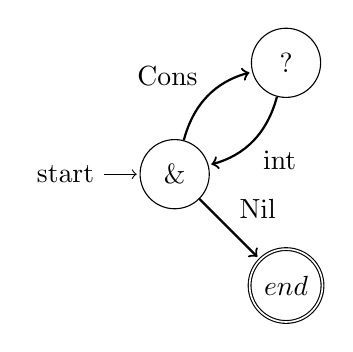
\begin{tikzpicture}[shorten >=1pt,node distance=2cm,on grid,auto] 
   \node[state,initial] (choice)   {$\&$}; 
   \node[state] (input) [above right=of choice] {$?$}; 
   \node[state,accepting] (end) [below right=of choice] {$end$}; 

   \path[edge] (choice) to[bend left] node {Cons} (input);
   \path[edge] (input) to[bend left] node {int} (choice);
   \path[edge] (choice) edge node {Nil} (end);
   
  \end{tikzpicture}
\end{center}

%%% Local Variables:
%%% mode: latex
%%% TeX-master: "cfst-inforum18"
%%% End:

Deste modo, podemos verificar que é possível enviar listas de uma maneira segura recorrendo a tipos de sessão. Contudo, estes tipos têm limitações na sua estrutura que tornam impossível a descrição eficiente de serializações de dados estruturados em forma de árvore \cite{ref-cfst}.
%\cite{ref_Thiemann_Vasconcelos_CFST}.

O exemplo proposto por Thiemann e Vasconcelos \cite{ref-cfst}
mostra a limitação dos tipos de sessão, formalizando o envio de árvores binárias num canal de comunicação. Neste exemplo, à semelhança do anterior, definiu-se o tipo recursivo para as árvores:
\begin{lstlisting}
	type Tree = Leaf | Node int Tree Tree
\end{lstlisting}
Para serializar esta estrutura é necessário percorrê-la numa determinada ordem transmitindo os valores das folhas (\lstinline"Leaf"), dos nós (\lstinline"Node") e dos inteiros. A sequência de operações para serializar esta árvore pode ser descrita pela seguinte gramática livre de contexto:
\begin{lstlisting}
	N ::= Leaf | Node int N N
\end{lstlisting}
Se observarmos a linguagem produzida pelo não terminal N podemos constatar que é livre de contexto mas não é regular, contrariamente à linguagem do exemplo da lista, que é descrita pela seguinte expressão regular $(\&\mbox{Cons}\,.\,?\mbox{int})^{*}\,\&\mbox{Nil}$. Como cada tipo de sessão tradicional tem como linguagem a união de uma linguagem regular com uma linguagem $\omega$-regular, que descreve as sequências finitas e infinitas admitidas pelo tipo, podemos concluir que não é possível serializar uma árvore recorrendo a tipos de sessão.

A linguagem que apresentamos é concorrente e explicitamente tipificada, onde os processos comunicam exclusivamente por troca de mensagens cujos protocolos são definidos pelos tipos de sessão livres de contexto apresentados por Thiemann e Vasconcelos \cite{ref-cfst}.


%%% Local Variables:
%%% mode: latex
%%% TeX-master: "cfst-inforum18"
%%% End:
